\documentclass[12pt]{article}
 
\usepackage[margin=1in]{geometry} 
\usepackage{amsmath,amsthm,amssymb}
\usepackage{graphicx}
\usepackage{tikz}
\usepackage{tikz-qtree}
\usepackage{wrapfig}
\usetikzlibrary{calc,patterns,angles,quotes}
 
\newcommand{\N}{\mathbb{N}}
\newcommand{\Z}{\mathbb{Z}}
\newcommand{\R}{\mathbb{R}}
\newcommand{\C}{\mathbb{C}}

\usepackage{mathtools}

%\DeclarePairedDelimiter\ceil{\left\lceil}  {\right\rceil}
%\DeclarePairedDelimiter\floor{\left\lfloor}{\right\rfloor}
 
\usepackage{amsthm}
\newtheorem{proposition}{Proposition}
\newtheorem{question}{Question}                                                                                                                                                                                          
 
\begin{document}
 
\title{Solutions to Exercise Sheet 4}
\author{Leif Van Holland \\ \\
\textsc{Discrete and Computational Geometry}}

\maketitle

\section*{Exercise 10}

\section*{Exercise 11}

Normalizing the height of the bounding box of all points to 1, we get the following coordinates by measurement
\[ p_1 = (0.04, 1),\: p_2 = (0,0.47),\: p_3=(0.04,0.42),\: p_4=(2.88,0.39) \]
\[ p_5=(3.35, 0.12),\: p_6 = (3.3, 0.05),\: p_7=(2.72, 0) \]

The resulting bounding boxes for the split-tree are visualized in the following picture:

\begin{figure}[h!]
\centering
\begin{tikzpicture}[xscale=4,yscale=4]
\coordinate (p1) at (0.04,1);
\coordinate (p2) at (0,0.47);
\coordinate (p3) at (0.04,0.42);
\coordinate (p4) at (2.88,0.39);
\coordinate (p5) at (3.35,0.12);
\coordinate (p6) at (3.3,0.05);
\coordinate (p7) at (2.72,0);

\filldraw[black] (p1) circle (0.5pt) node[anchor=south] {$p_1$};
\filldraw[black] (p2) circle (0.5pt) node[anchor=south] {$p_2$};
\filldraw[black] (p3) circle (0.5pt) node[anchor=west] {$p_3$};
\filldraw[black] (p4) circle (0.5pt) node[anchor=south] {$p_4$};
\filldraw[black] (p5) circle (0.5pt) node[anchor=south] {$p_5$};
\filldraw[black] (p6) circle (0.5pt) node[anchor=north] {$p_6$};
\filldraw[black] (p7) circle (0.5pt) node[anchor=south] {$p_7$};

\draw (0,0.42) -- (p3) -- (p1) -- (0,1) -- (0,0.42);
\draw (0,0.42) -- (p3) -- (0.04, 0.47) -- (p2) -- (0,0.42);
\draw (p7) -- (3.35,0) -- (3.35, 0.39) -- (2.72, 0.39) -- (p7);
\draw (p7) -- (2.88, 0) -- (p4) -- (2.72,0.39) -- (p7);
\draw (p6) -- (3.35,0.05) -- (p5) -- (3.3, 0.12) -- (p6); 

\end{tikzpicture}
\end{figure}

This in turn creates the following split-tree:

\begin{figure}
    \centering
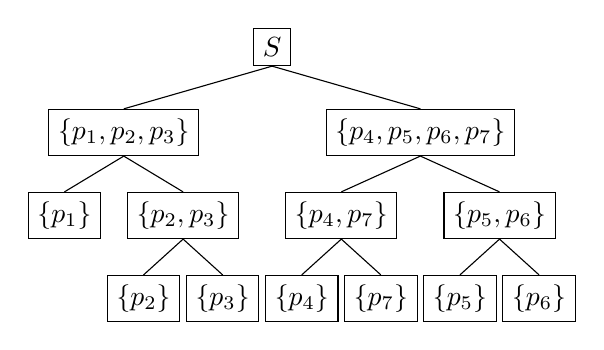
\begin{tikzpicture}[every node/.style={rectangle, draw=black}]
\Tree [.$S$
    [.$\{p_1,p_2,p_3\}$
        [.$\{p_1\}$ ]
        [.$\{p_2,p_3\}$
            [.$\{p_2\}$ ]
            [.$\{p_3\}$ ]
        ]
    ]
    [.$\{p_4,p_5,p_6,p_7\}$
        [.$\{p_4,p_7\}$
            [.$\{p_4\}$ ]
            [.$\{p_7\}$ ]
        ]
        [.$\{p_5,p_6\}$
            [.$\{p_5\}$ ]
            [.$\{p_6\}$ ]
        ]
    ]
]
\end{tikzpicture}
\end{figure}
\end{document}